%\documentclass[a4paper,10pt]{amsart}
\documentclass[a4paper,10pt]{article}
\usepackage[latin1]{inputenc}
\usepackage[spanish]{babel}
\usepackage[dvips]{epsfig}
\usepackage{graphicx}
\usepackage{verbatim}
\usepackage{amssymb}
\usepackage{amsmath}
\usepackage{amsfonts}

\title{Trabajo Pr\'actico Final\\ Simulaci\'on de Sistemas\\ (72.25)}

\author{
Abramowicz Pablo\\
Gomez Vidal Maximiliano\\
Sessa Carlos\\
Villa Fernandez Santiago\\
}

\begin{document}
\maketitle

\section*{Item a}

\subsection*{Tiempo entre arribos}


Para modelar el intervalo de tiempos entre arribos se cuenta con mediciones del
horario en que los clientes llegaron al sistema. La regla de
Sturges para la elecci\'on de la cantidad de intervalos de clase 
aconseja utilizar $1 + \log_2 n$ intervalos, siendo $n$
la cantidad de datos. De esta manera se obtiene que se requieren $7.644$ intervalos,
utilizando en este caso $8$. 

\begin{figure*}[hp]
\centering
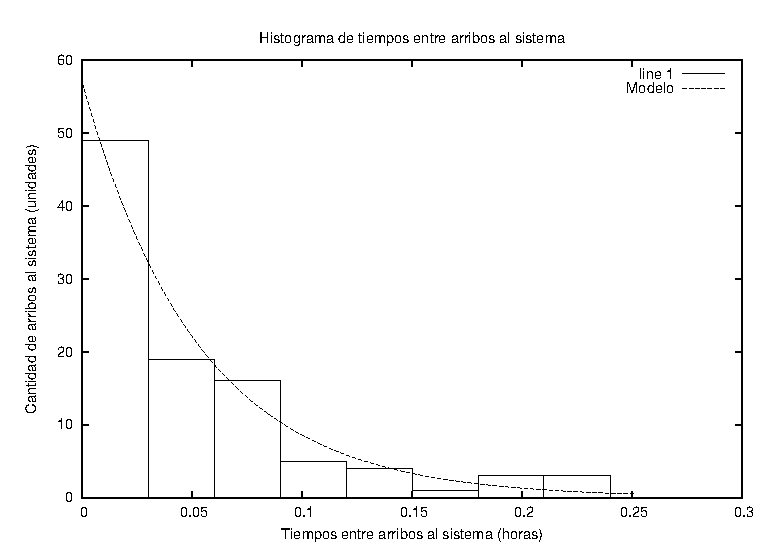
\includegraphics{graficos/histograma_llegadas.eps}
\caption{Tiempo entre arribos al sistema}
\label{fig:tiempoentrearribos}
\end{figure*}


En la figura ~\ref{fig:tiempoentrearribos} se observa el histograma con los
intervalos de tiempo entre arribos. Se percibe que los datos tienden a estar
distribuidos en forma exponencial. Se realiza un test de bondad de ajuste
$\chi^2$ para comprobarlo.


Se estima el valor medio de la muestra obteni\'endose 
$\lambda = 18.939$ [clientes/hora],
con un estad\'istico chi-cuadrado de valor $\chi_0^2 = 11.943$. 
El valor cr\'itico para $7$ grados de libertad con un nivel
de significaci\'on del $5\%$ resulta $\chi_{7,0.05}^2 = 14.067$. Por lo tanto,
no puede refutarse la hip\'otesis de que los datos provengan de una distribuci\'on 
exponencial.

\begin{figure*}[hp]
\centering
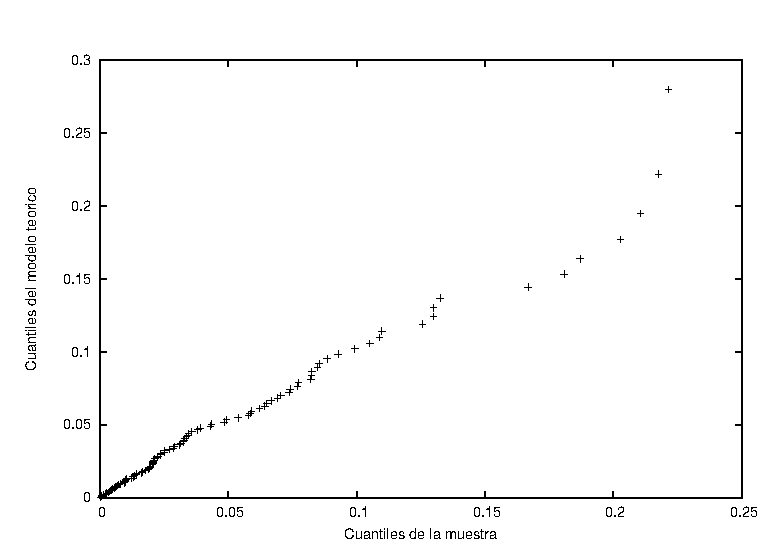
\includegraphics{graficos/plot_qq_llegadas.eps}
\caption{Plot Q-Q del tiempo entre arribos al sistema}
\label{fig:qqarribos}
\end{figure*}


En la figura ~\ref{fig:qqarribos} se muestra un plot Q-Q. Se visualiza que los cuantiles se encuentran
alineados sobre una recta de pendiente unitaria, en especial para valores
peque\~nos. De este an\'alisis se desprende que la distribuci\'on de la
muestra es muy similar a la exponencial.


Realizando un test de uniformidad
Kolmogorov-Smirnov sobre los tiempos de arribos se obtiene un estad\'istico
de $D = 0.12686$, considerando nuevamente los datos agrupados en $8$ clases. 
El valor cr\'itico para un nivel de significaci\'on del $5\%$ 
se obtiene de tabla y resulta $D_{7, 0.05} = 0.4361$.
Puesto que $D_{7,0.05} > D$ no se puede afirmar que los datos
no provengan de una distribuci\'on exponencial. 


Debido a que los tests resultaron satisfactorios, se supone para las 
simulaciones que los se encuentran distribuidos exponencialmente con media
$\lambda = 18.939$ [clientes/hora].


\subsection*{Tiempo de atenci\'on de la estaci\'on E3}


El resultado de aplicar la regla de Sturges indica utilizar $8.644$ intervalos
de clase. Empleando adem\'as la regla de Nu\~nez se opta por utilizar $8$ 
intervalos de clase.

\begin{figure*}[hp]
\centering
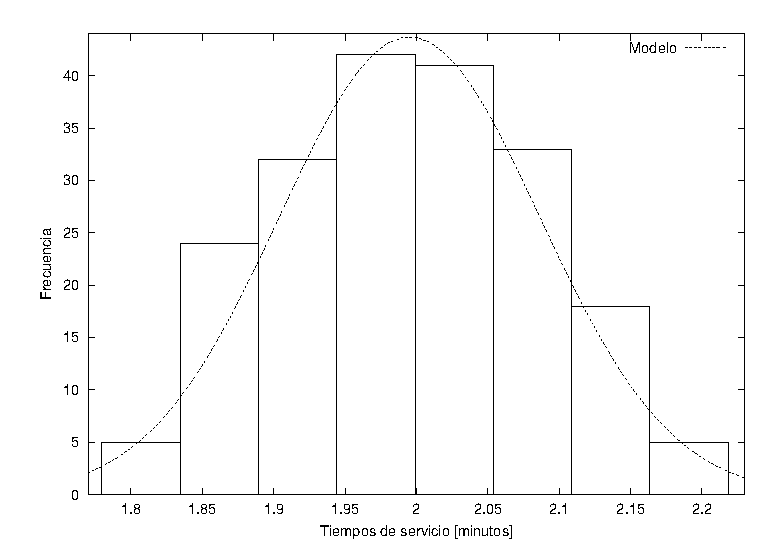
\includegraphics{graficos/histograma_e3.eps}
\caption{Tiempo de atenci\'on de la estaci\'on E3}
\label{fig:tiempoatencione3}
\end{figure*}


El histograma de tiempo de atenci\'on dado en la figura 
 ~\ref{fig:tiempoatencione3}
muestra que los datos presentan una distribuci\'on aproximadamente
normal.

La estimaci\'on de la media resulta $\mu = 1.9952 $ y la varianza tiene un valor
$\sigma^2 = 0.00832$. Se realiza el test de bondad de ajuste $\chi^2$ para
analizar si es razonable suponer que la distribuci\'on observada es normal.

\begin{figure*}[hp]
\centering
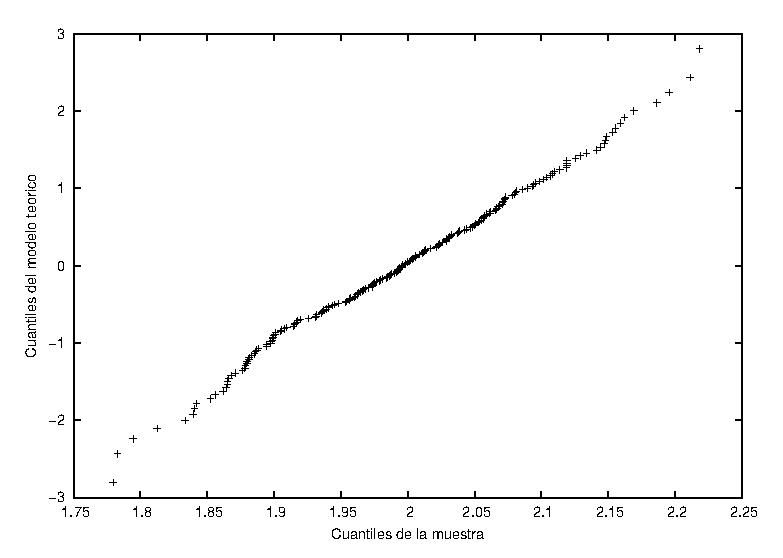
\includegraphics{graficos/plot_qq_e3.eps}
\caption{Plot Q-Q del tiempo de atenci\'on en la facilidad E3}
\label{fig:qqe3}
\end{figure*}


El valor del estad\'istico es $\chi_0^2 = 4.7492$, resultando menor que el valor 
cr\'itico obtenido por tablas para $7$ grados de libertad con un nivel de 
significaci\'on del $5\%$, cuyo valor es $\chi_{7,0.05}^2 = 14.067$. En
consecuencia, no se refuta la hip\'otesis de que los datos provengan de una 
distribuci\'on normal. En la figura  ~\ref{fig:qqe3} se observa el plot Q-Q comparando
ambas distribuciones.


\section*{\underline{Item b}}
\section*{\underline{Item c}}
%Indicar los tipos de eventos y el espacio de eventos
Como se observ\'o anteriormente las colas involucradas son
$S = \{R, E1, E3, OFT, PSF, E2, C\}$.\\
Todas las colas del sistema se modelan con capacidad infinita y un
comportamiento \textbf{FIFO} (\textit{first in- first out}), salvo la cola $E3$
donde se considera que los clientes que todav\'ia no alcanzan a llenar el
formulario, son desplazados un lugar hacia atras en dicha cola.\\
Los eventos para cada cola del sistema son la llegada y la salida de un cliente.
Utilizando subindices para nombrar los eventos de cada cola, el espacio de
eventos ($E$) del sistema resulta:\\
$$E = \{Ra , Rp , E1a , E1p , E3a , E3p , OFTa , OFTp , PSFa , PSFp , E2a , E2p , Ca , Cp \}$$\\
Donde el sub\'indice \textit{a} indica la llegada de un cliente a la cola y el
sub\'indice \textit{p} indica la partida de un cliente de la cola.

\section*{\underline{Item d}}
\section*{\underline{Item e}}
\section*{\underline{Item f}}
\section*{\underline{Item g}}



\end{document}
